\documentclass[withindex,glossary]{cam-thesis}
% Citations using numbers\documentclass{standalone}
\usepackage[T1]{fontenc}                
\usepackage{tikz}
\usepackage{tikz-qtree,tikz-qtree-compat}
\usetikzlibrary{calc}
\usepackage{multirow}
\usepackage{array}
\usepackage[utf8]{inputenc}             
\usepackage{tikz}
\usepackage{float}
\usepackage{forest}
\usepackage{blindtext}
\usepackage{tabularx}
\usepackage{subfigure}
\usepackage{pgfplots}
\pgfplotsset{compat=1.14}
\usepackage[utf8]{inputenc}
\usepackage{amsmath, amssymb, latexsym}
\usepackage{tikz}
\usetikzlibrary{decorations.pathreplacing}
\usetikzlibrary{fadings}
\usetikzlibrary{shapes,arrows,fit,calc,positioning}
\tikzset{box/.style={draw, diamond, thick, text centered, minimum height=0.5cm, minimum width=1cm}}
\tikzset{line/.style={draw, thick, -latex'}}
% FOR MATHS
\usepackage[numbers]{natbib}
\usepackage{amsmath}
\usepackage{amssymb}
\newcommand{\R}{\mathbb{R}}
\newcommand{\argmax}{\arg\!\max}
% FOR ALGORITHMS
\usepackage{algorithm}
\usepackage[noend]{algpseudocode}
%% The title of the thesis:

\title{Comparing Machine Learning Techniques for Mobility
Graph Classification}
\author{Miteyan Patel}

\college{Robinson College}
\collegeshield{CollegeShields/Robinson}
\submissiondate{20th May, 2018}
%% Declaration date:
\date{December, 2017}
%% PDF meta-info:
\subjectline{Computer Science}
%% Abstract:
%%
%% Acknowledgements:
% \acknowledgements{%
%   My acknowledgements ...
% }
%% Glossary [optional]:
%%
%% Contents:
%%
\begin{document}

%% Title page, abstract, declaration etc.:
%% -    the title page (is automatically omitted in the technical report mode).
\frontmatter{}
%% Thesis body:
%%
\chapter{Introduction}
This dissertation proposes an Android application that is capable of locally inferring the demographic class of its user. A mobility graph constructed from the user's location data is used as input into a trained Random Forest model.\\
This dissertation describes the preparation work, implementation, analysis and evaluation of supervised machine learning algorithms and their application to mobility graphs and local inferences on Android. The machine learning algorithms either apply the location graphs  directly to a Convolutional Neural Network architecture or take features from the graphs and then apply standard supervised learning algorithms such as Naive Bayes, Support Vector Machines, Decision Trees, Random Forests and Deep Neural Networks. 

\section{Motivation}
Machine learning techniques typically use structured, organised data, which restricts the domain of data that can be used since unstructured data does not have a pre-defined data model and arises commonly in reality, for example in the form of social networks, web networks, audio or video. The increasing availability of unstructured data has  presented the challenge of extracting features from this information-dense data to allow for a classification to take place. This leads to an interesting classification problem in the form of classifying the demographic label of mobility graphs, which are graphs constructed from location data. Nodes in the graph correspond to the locations visited by the user and edges as connections between these locations. The differences in demographics between users could lead to a difference in their movement patterns which we could exploit using machine learning classifiers. These mobility graphs are used to train a collection of supervised machine learning algorithms, including the use of a new Convolutional Neural Network architecture~\cite{CNN1}, from which the best model is evaluated and transferred onto an Android application to make inferences from the location data collected from the user. The mobility graphs are constructed from datasets containing demographic labels such as gender or occupation and the machine learning models will be optimised to determine the most suitable model to export to an Android application. A mobile application was created to collect and cluster the location data into graphs for use by the most successfully evaluated of these techniques to locally infer the class of the user.\\
This application can be used as a framework which uses location data to infer the class of a user, for example whether or not users have neurological diseases such as Alzheimer’s Disease, which has been known to alter the movement patterns of its sufferers. Another application of this project is dealing with the use of machine learning algorithms locally on mobile devices without the need to send any data to the server and risk the leaking of sensitive information such as their locations collected. It also does not have to deal with the taking data out of its legislative data protection borders.\\ 
\section{Related Work}
Convolutional Neural Networks~\citep{CNN1} have been applied to classify unstructured graph data such as text categorisation, synthetic random graphs and even graphs constructed from structured image data to a high performance. However, mobility graphs have not been classified before using this or any similar algorithms.\\
Smart phones already use machine learning locally to do various tasks from predictive typing on keyboards to classifying images into folders and making suggested actions of highlighted text. Wearable technology like smart watches also make use of passive data collected from the sensors throughout the day to infer if the user could have an underlying disease~\cite{apple}.

\chapter{Preparation}
My preparation consisted of learning about supervised machine learning algorithms in order to optimize them. Understanding of techniques for the evaluation of the machine learning was paramount in ensuring the correct algorithm is chosen. Research in graph theory was done to find the most relevant features that could be used to classify graphs and to find techniques such as clustering to create the graphs from the raw location data.
\section{Clustering}
Clustering involves grouping data into sets in such a way that objects in the same group are more similar to each other than to those in other groups. The location data needs to be grouped so that all nearby locations are in the same cluster to represent a single place the user has visited. The user may not move to a new location every recording and so this will reduce the number of locations visited in the graph and increase the edge weight between the nodes. In theory make the graphs simpler to process whilst conveying more information than a graph simply made of each location value as a node. A useful algorithm for this is the DBSCAN algorithm described in section 2.1.1 since it is efficient enough to work on Android phones and does not need the number of clusters to be specified as with k-means clustering, a popular clustering algorithm.
\subsection{Density Based Spatial Clustering Of Applications With Noise}
DBSCAN is a density-based clustering algorithm: given a set of points in space, it groups together points with many nearby neighbours in a cluster, and marks distant points too far away as noise. It takes two parameters, a minimum distance $\epsilon$ that a point needs to be from another point to be considered its neighbour and the minimum number of points needed to form a cluster, minPoints. If there are more than minPoints other points within $\epsilon$ from a random point, a cluster is formed. The cluster is expanded by checking the new points and if they have more than minPoints points within $\epsilon$ the cluster is grown recursively. The process is repeated until the cluster cannot be expanded. A point with fewer than minPoints is considered as an outlier or "noise point" and does not belong to any cluster.
\begin{algorithm}
\caption{DBSCAN algorithm for clustering locations}
\label{alg:erdos}
\begin{algorithmic}[1]
\Procedure{$cluster(locations, \epsilon, minPoints)$}{}
\State clusters = []
\For {randomLocation in unvisited(locations)}
\State cluster = $\emptyset$
		\While {numNeighbours(randomLocation, $\epsilon$) > minPoints}
        	\State $cluster \gets neighbours(randomPoint, \epsilon)$
            \State $randomLocation \gets cluster.nextPoint$
        \EndWhile
		\State $clusters \gets cluster$
\EndFor
\State \textbf{return} clusters
\EndProcedure
\end{algorithmic}
\end{algorithm}

\section{Graph Theory}
A graph is a set of nodes that are related to each other and edges that connected these. To use graphs constructed from the user location data as inputs into the traditional supervised machine learning algorithms, the features belonging to the graphs must be extracted. I will explain some of the graph features we can extract to distinguish between graphs belonging to different classes. Some of these features are defined for each node in the graph and so the mean and variances of these  vectors are used as features.
\subsection{Graph Features}
\begin{description}
\item [Number of nodes and edges:] the number of nodes and edges in the graph.
\item [Max degree:] the maximum number of neighbours any node in the graph has.
\item [Density:] a graph's density is defined as: $$\frac{|Edges|}{|Nodes|(|Nodes| - 1)}$$ for directed graphs, a dense graph is a graph in which the number of edges is close to the maximal number of edges possible. 
\item [Eccentricity:] eccentricity of a node is the maximum distance to any other node in the graph. This is a vector as it is defined for each node in the graph and so the mean and variance of the eccentricity are used as scalar valued features.
\item [Diameter:] the greatest distance between any two nodes in the graph, also the max eccentricity in the graph.
\item [Radius:] the minimum eccentricity value from graph.
\item [Centre Size:] the size of the centre of a graph. The centre of a graph is the set of all nodes in the graph which have eccentricity equal to the radius of the graph. 
\item [Shortest Path Length:] the average and variance of the shortest path between all pairs of nodes in the graph. 
\item [Clustering Coefficient:] measure of the degree to which nodes in a graph tend to cluster together. 
\item [Betweenness Centrality:]  the betweenness centrality for each vertex is the number of  shortest paths that pass through the vertex. The shortest path between the vertices is one where the sum of the weights of the edges is minimized.
\item [Edge Betweenness Centrality:] vector containing the fraction of shortest paths each edge belongs to. The mean and variance of these are extracted as features.
\item [PageRank:] computes a ranking of the nodes in the graph based on the structure of the incoming links.
\end{description}
\section{Supervised Machine Learning}
Supervised learning algorithms are used to learn the mapping function from input data to the class it belongs to. Input feature vectors $\mathbf{x} \in \R^{m}$ are associated with a label y. In classification problems, y represents one of the possible output classes $\mathbf{C} = \{C_1, ..., C_k\}$.
 A training set is composed of n such training examples: $$\mathbf{s} = [(\mathbf{x_1}, y_1) (\mathbf{x_2}, y_2) ... (\mathbf{x_n}, y_n)]$$
The goal is to approximate the mapping function, the hypothesis $h:  \R^{m} \rightarrow \mathbf{C}$, so when there is new input data $\mathbf{x}$, the output class for that data can be predicted. The following sections explain the theory behind the algorithms I will be using.
\subsection{Neural Networks}
Based on the extravagantly complex neuron networks in the brain, a type of supervised learning algorithm commonly used is the neural network. Although they are an oversimplification of the biological neural networks, they offer a very successful technique for regression and classification problems. It defines some function $f(\mathbf{x};\mathbf{w}, \mathbf{b}$), dependent on its architecture to approximate the hypothesis, where $\mathbf{x}$ is the input vector, $\mathbf{w}$ and $\mathbf{b}$ are the weights and biases in the network. The neural network over successive iterations of the training algorithm learns the values of weights and biases by minimising a loss function. A loss function defines the measure of the error when estimating y from $\mathbf{x}$ to its actual class. The following sections describe the components of the Neural Network. \\
\subsubsection{Perceptron}
\tikzset{basic/.style={draw,text width=1em,text badly centered}}
\tikzset{input/.style={basic,circle}}
\tikzset{weights/.style={basic,rectangle}}
\tikzset{functions/.style={basic,circle}}
\begin{figure}[H]
\centering
$$
\begin{tikzpicture}
\node[functions] (center) {};
\node[below of=center,font=\scriptsize,text width=4em] {Activation function $\sigma$};
\draw[thick] (0.5em,0.5em) -- (0,0.5em) -- (0,-0.5em) -- (-0.5em,-0.5em);
\draw (0em,0.75em) -- (0em,-0.75em);
\draw (0.75em,0em) -- (-0.75em,0em);
\node[right of=center] (right) {};
\path[draw,->] (center) -- (right);
\node[functions,left=3em of center] (left) {$\sum$};
\path[draw,->] (left) -- (center);
\node[weights,left=3em of left] (2) {$w_2$} -- (2) node[input,left of=2] (l2) {$x_2$};
\path[draw,->] (l2) -- (2);
\path[draw,->] (2) -- (left);
\node[below of=2] (dots) {$\vdots$} -- (dots) node[left of=dots] (ldots) {$\vdots$};
\node[weights,below of=dots] (n) {$w_n$} -- (n) node[input,left of=n] (ln) {$x_n$};
\path[draw,->] (ln) -- (n);
\path[draw,->] (n) -- (left);
\node[weights,above of=2] (1) {$w_1$} -- (1) node[input,left of=1] (l1) {$x_1$};
\path[draw,->] (l1) -- (1);
\path[draw,->] (1) -- (left);
\node[weights,above of=1] (0) {$w_0$} -- (0) node[input,left of=0] (l0) {$1$};
\path[draw,->] (l0) -- (0);
\path[draw,->] (0) -- (left);
\node[below of=ln,font=\scriptsize] {Inputs};
\node[below of=n,font=\scriptsize] {Weights};
\end{tikzpicture}
$$
\caption{A diagram of a perceptron showing the action of a cross product applied to the input vector \textbf{x} and weights \textbf{w}, followed by an activation function such as the sigmoid. } \label{fig:Perceptron}
\end{figure}
A perceptron, shown in figure \ref{fig:Perceptron}, on its own is a linear classifier which makes predictions based on a linear combination of the weights and input features. The output of the perceptron is the cross product of the weights and the inputs into it followed by a pass through the activation function, which is used to normalise the output from the perceptron.  The constant-valued input 1 for $x_0$ is known as a bias input, which is weighted by a bias weight variable, $w_0$. This allows the output of the network to be shifted left or right to maximise the accuracy and range of values that can be modelled by the perceptron. 
$$
h(w; x)= \sigma (\sum_{i=0}^{n}w_i x_i) = \sigma (\bf{w}^T \bf{x})
$$
\subsubsection{Multi-layered Perceptron}
Perceptrons on their own are not powerful enough to generalise to more complex non-linear functions. A multilayer perceptron is a collection of fully connected perceptrons, consisting of at least three layers connected by non-linear activation functions to generate non-linearity. Every perceptron is connected to at least one in the layer in front with a weight, shown in figure \ref{fig:multilayer-perceptron}. Learning occurs in the perceptron by changing connection weights after processing the training data, based on the amount of error in the output compared to the expected result, through backpropagation. 
\begin{figure}[H]
	\centering
	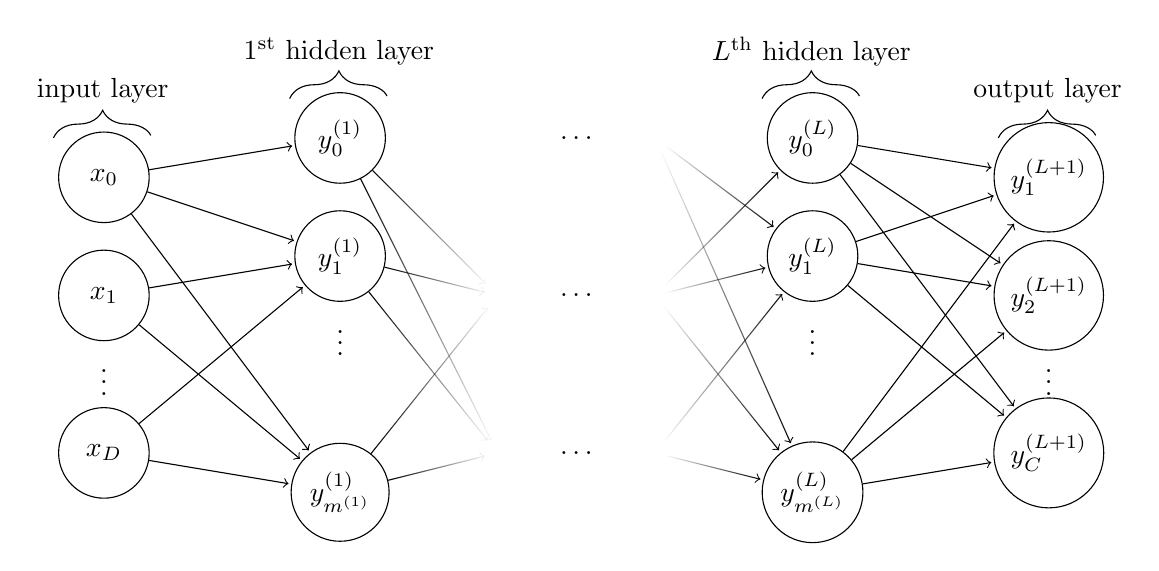
\begin{tikzpicture}[shorten >=1pt]
		\tikzstyle{unit}=[draw,shape=circle,minimum size=1.15cm]
		%\tikzstyle{hidden}=[draw,shape=circle,fill=black!25,minimum size=1.15cm]
		\tikzstyle{hidden}=[draw,shape=circle,minimum size=1.15cm]

		\node[unit](x0) at (0,3.5){$x_0$};
		\node[unit](x1) at (0,2){$x_1$};
		\node at (0,1){\vdots};
		\node[unit](xd) at (0,0){$x_D$};

		\node[hidden](h10) at (3,4){$y_0^{(1)}$};
		\node[hidden](h11) at (3,2.5){$y_1^{(1)}$};
		\node at (3,1.5){\vdots};
		\node[hidden](h1m) at (3,-0.5){$y_{m^{(1)}}^{(1)}$};

		\node(h22) at (5,0){};
		\node(h21) at (5,2){};
		\node(h20) at (5,4){};
		
		\node(d3) at (6,0){$\ldots$};
		\node(d2) at (6,2){$\ldots$};
		\node(d1) at (6,4){$\ldots$};

		\node(hL12) at (7,0){};
		\node(hL11) at (7,2){};
		\node(hL10) at (7,4){};
		
		\node[hidden](hL0) at (9,4){$y_0^{(L)}$};
		\node[hidden](hL1) at (9,2.5){$y_1^{(L)}$};
		\node at (9,1.5){\vdots};
		\node[hidden](hLm) at (9,-0.5){$y_{m^{(L)}}^{(L)}$};

		\node[unit](y1) at (12,3.5){$y_1^{(L+1)}$};
		\node[unit](y2) at (12,2){$y_2^{(L+1)}$};
		\node at (12,1){\vdots};	
		\node[unit](yc) at (12,0){$y_C^{(L+1)}$};
		
		\draw[->] (x0) -- (h10);
		\draw[->] (x0) -- (h11);
		\draw[->] (x0) -- (h1m);

		\draw[->] (x1) -- (h11);
		\draw[->] (x1) -- (h1m);

		\draw[->] (xd) -- (h11);
		\draw[->] (xd) -- (h1m);

		\draw[->] (hL0) -- (y1);
		\draw[->] (hL0) -- (yc);
		\draw[->] (hL0) -- (y2);

		\draw[->] (hL1) -- (y1);
		\draw[->] (hL1) -- (yc);
		\draw[->] (hL1) -- (y2);

		\draw[->] (hLm) -- (y1);
		\draw[->] (hLm) -- (y2);
		\draw[->] (hLm) -- (yc);
		\draw[->,path fading=east] (h10) -- (h21);
		\draw[->,path fading=east] (h10) -- (h22);
		
		\draw[->,path fading=east] (h11) -- (h21);
		\draw[->,path fading=east] (h11) -- (h22);
		
		\draw[->,path fading=east] (h1m) -- (h21);
		\draw[->,path fading=east] (h1m) -- (h22);
		
		\draw[->,path fading=west] (hL11) -- (hL0);
		\draw[->,path fading=west] (hL10) -- (hL1);
		\draw[->,path fading=west] (hL11) -- (hL1);
		\draw[->,path fading=west] (hL12) -- (hL1);
		
		\draw[->,path fading=west] (hL10) -- (hLm);
		\draw[->,path fading=west] (hL11) -- (hLm);
		\draw[->,path fading=west] (hL12) -- (hLm);
		
		\draw [decorate,decoration={brace,amplitude=10pt},xshift=-4pt,yshift=0pt] (-0.5,4) -- (0.75,4) node [black,midway,yshift=+0.6cm]{input layer};
		\draw [decorate,decoration={brace,amplitude=10pt},xshift=-4pt,yshift=0pt] (2.5,4.5) -- (3.75,4.5) node [black,midway,yshift=+0.6cm]{$1^{\text{st}}$ hidden layer};
		\draw [decorate,decoration={brace,amplitude=10pt},xshift=-4pt,yshift=0pt] (8.5,4.5) -- (9.75,4.5) node [black,midway,yshift=+0.6cm]{$L^{\text{th}}$ hidden layer};
		\draw [decorate,decoration={brace,amplitude=10pt},xshift=-4pt,yshift=0pt] (11.5,4) -- (12.75,4) node [black,midway,yshift=+0.6cm]{output layer};
	\end{tikzpicture}
	\caption[Network graph for a $(L+1)$-layer perceptron.]{Network graph of a $(L+1)$-layer perceptron with $D$ input units and $C$ output units. The $l^{\text{th}}$ hidden layer contains $m^{(l)}$ hidden units.}
	\label{fig:multilayer-perceptron}
\end{figure}
\subsubsection{Activation Functions}
Activation functions decide whether or not a neuron should be activated or transmit information. 
The activation function needs to be non-linear, which can be proved to be a universal function approximator for a two-layered network and allows for errors to be backpropagated more easily~\cite{approximator}. The Sigmoid function is commonly used in neural networks and activates the neuron when the value is more than 0.5. Rectified Linear Units (ReLUs) are used in Convolution Neural Networks, which are in practice more effective than the sigmoid or tanh functions. However at the negative side of the graph, the gradient is zero, which means for activations in that region, the gradient is zero and the weights are not updated during back propagation. This can create dead neurons which never get activated. The leaky ReLU solves this by replacing the horizontal section by a line with a small gradient so there are no more dead neurons for better classification. 
\begin{figure}[H]
	\centering
	\subfigure[Logistic sigmoid]{
    		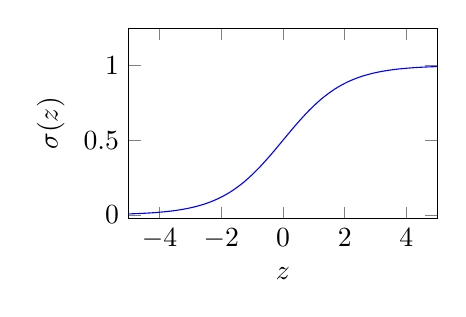
\begin{tikzpicture}
			\begin{axis}[width=5.5cm,height=4cm,ylabel=$\sigma(z)$,xlabel=$z$,ymin=-.025,ymax=1.25,xmin=-5,xmax=5]
				\addplot[blue,smooth] {1/(1+exp(-x))};
			\end{axis}
		\end{tikzpicture}
	}
	\subfigure[Hyperbolic tangent]{
		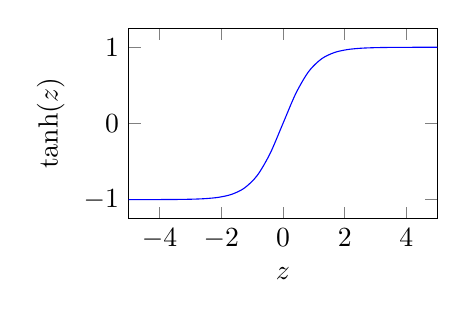
\begin{tikzpicture}
			\begin{axis}[width=5.5cm,height=4cm,ylabel=$\tanh(z)$,xlabel=$z$,ymin=-1.25,ymax=1.25,xmin=-5,xmax=5]
				\addplot[blue,smooth] {tanh(x)};
			\end{axis}
		\end{tikzpicture}
	}
    \subfigure[ReLU]{
		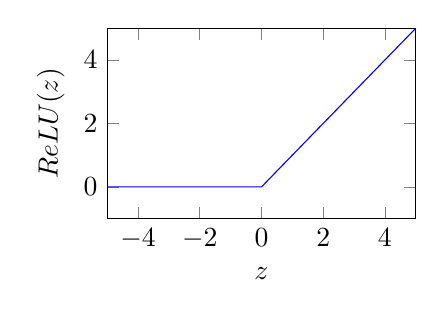
\begin{tikzpicture}
			\begin{axis}[width=5.5cm,height=4cm,ylabel=$ReLU(z)$,xlabel=$z$,ymin=-1,ymax=5,xmin=-5,xmax=5]
				\addplot[blue] {max(0,x)};
			\end{axis}
		\end{tikzpicture}
	}
    \subfigure[Leaky ReLU]{
		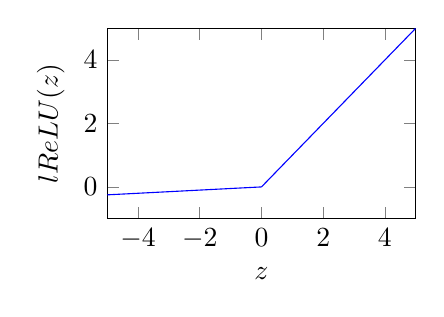
\begin{tikzpicture}
			\begin{axis}[width=5.5cm,height=4cm,ylabel=$lReLU(z)$,xlabel=$z$,ymin=-1,ymax=5,xmin=-5,xmax=5]
				\addplot[blue] {max(0.05*x,x)};
			\end{axis}
		\end{tikzpicture}
	}
    	\caption[Sigmoidal activation functions.]{Commonly used activation functions including the logistic sigmoid $\sigma(z)$, the hyperbolic tangent $tanh(z)$, ReLU and leaky ReLU.}
    	\label{fig:sigmoid-tanh}
\end{figure}
\subsubsection{Gradient Descent}
A common method for training a perceptron is gradient descent. It is an optimisation technique to reduce the error over the whole network to improve the mapping between the input features and the output classes to better improve the fit of the network to the training data to better improve its predictions for the test data. The differentiable error term E(\textbf{w}) is defined, which is the squared difference between what the network is currently outputting $h(\mathbf{w,x_i}$) for the training data $\mathbf{x_i}$ and the actual class that data belongs to $y_i$:
$$
E(\textbf{w}) = \sum_{i=1}^{n} {(y_i - h(\mathbf{w};\mathbf{x}_i))}^2
$$
We try to minimise the error term for the whole network $E(\textbf{w})$ by tending the weights for the network $\textbf{w}$ to reduce the error by updating the weights as follows:
$$
\mathbf{w}_{t+1} = \mathbf{w}_t - \eta \frac{\partial E(\textbf{w})}{\partial \mathbf{w}}
$$
The learning rate, $\eta$, is a parameter which is a small positive number which controls rate at which the weights are updated. It is a trade-off between training time with a large learning rate and greater accuracy gained from using a smaller learning rate. In practice an adaptive learning rate is used which slowly decreases as the weights converge to reducing the error rate. This prevents getting stuck in a local minima.  The partial differential term is the direction of the steepest decrease in error and so the weight is updated to decrease the error. For our error term where $\mathbf{x}_{i}^j$ is the jth element of $\mathbf{x}_i$ we have:
$$
\frac{\partial E(\textbf{w})}{\partial  w_j} = -2 \sum_{i=1}^{n} \mathbf{x}_{i}^j (y_i - h(\mathbf{w};\mathbf{x}_i))
$$
So the gradient descent algorithm is as follows, initialise the weights $\mathbf{w}_0$ at the start to be random and update the weights as follows in our case:
$$
\mathbf{w}_{t+1} = \mathbf{w}_t + 2\eta  \sum_{i=1}^{n} \mathbf{x}_{i} (y_i - h(\mathbf{w};\mathbf{x}_i))
$$
We can stop once the error differences is smaller than a threshold value or a set number of iterations.
\subsubsection{Backpropagation}
The goal of backpropagation algorithm is to find a set of weights for the entire multi-layered perceptron network that minimises the error term using the gradient descent algorithm. To do this we need to find  $\frac{\partial E(\textbf{w})}{\partial \mathbf{w}}$ for the entire network which needs the calculation of $\frac{\partial E(\textbf{w})}{\partial {w}_{i,j}}$, for each weight ${w}_{i,j}$ in the network. The total error in the network produces over the entire training set is now defined as $E(\textbf{w}) =  \sum_{i=1}^{n} E_i(\mathbf{w})$ and $\frac{\partial E(\textbf{w})}{\partial \mathbf{w}} =  \sum_{i=1}^{n} 
\frac{\partial E_i(\mathbf{w})}{\partial \mathbf{w}}$
The algorithm consists of two phases, propagation and weight update:

\textbf{Propagation}
\begin{enumerate}
\item Propagate the input training vectors $\mathbf{x}_i$ through the network to generate the corresponding output values $h(\textbf{w};\mathbf{x}_i)$ for all nodes and the final output y.
\item Calculate the error term $E(\textbf{w})$ for the entire training set.
\item Propagate the actual output activations back through the network in reverse to generate the difference between the target and output values for all the neurons and weights.
% $$ or for the output layer as:
% $$
% \frac{\partial E(\textbf{w})}{\partial{w}_{i,j}^l} = \sum_{k=1}^{n} 
% \frac{\partial E_k(\textbf{w})}{\partial h(\textbf{w};\mathbf{x}_k)}  
% \frac{\partial{z}_{j}^{l+1}}{\partial{w}_{i,j}^l} 
% $$
\end{enumerate}
\textbf{Weight update}
\begin{enumerate}
\item Calculate the gradient for a weight ${w}_{i,j}^l$ in layer l, where ${z}_{j}^{l}$ is the output from the neuron j in layer l, in the general case as: 
$$
\frac{\partial E(\textbf{w})}{\partial{w}_{i,j}^l} = \sum_{k=1}^{n} 
\frac{\partial E_k(\textbf{w})}{\partial h(\textbf{w};\mathbf{x}_k)}  
\frac{\partial  h(\textbf{w};\mathbf{x}_k)}{\partial{z}_{j}^{l+1}} 
\frac{\partial{z}_{j}^{l+1}}{\partial{w}_{i,j}^l} 
$$
\item Update the weights using gradient descent as before with rule:
$$
{w}_{i,j}^l := {w}_{i,j}^l - \eta \frac{\partial E(\textbf{w})}{\partial{w}_{i,j}^l} 
$$
\end{enumerate}
\usetikzlibrary{matrix,chains,positioning,decorations.pathreplacing,arrows,calc}
\tikzset{
block/.style={
  draw,
  rectangle, 
  text width=3em, 
  text centered, 
  minimum height=8mm,     
  node distance=2.3em
  }, 
line/.style={draw}
}

\begin{figure}[H]
\centering
$$
\begin{tikzpicture}[
plain/.style={
draw=none,
fill=none,
},
net/.style={
matrix of nodes,
nodes={
draw,
circle,
inner sep=10pt
},
nodes in empty cells,
column sep=2cm,
row sep=-9pt
}, 
>=latex
]
\matrix[net] (mat)
{ 
|[plain]| \parbox{1cm}{\centering Input\\layer} & |[plain]| \parbox{1cm}{\centering     Hidden\\layer} & |[plain]| \parbox{1cm}{\centering Output\\layer} \\
& |[plain]| \\
|[plain]| & \\
& |[plain]| \\
|[plain]| & |[plain]| \\
& & \\
|[plain]| & |[plain]| \\
& |[plain]| \\
|[plain]| & \\
& |[plain]| \\
};
\foreach \ai [count=\mi ]in {2,4,...,10}
  \draw[<-] (mat-\ai-1) -- node[above] {Input \mi} +(-2cm,0);
\foreach \ai in {2,4,...,10}
{\foreach \aii in {3,6,9}
  \draw[->] (mat-\ai-1) -- (mat-\aii-2);
}
\foreach \ai in {3,6,9}
  \draw[->] (mat-\ai-2) -- (mat-6-3);
%\draw[->] (mat-6-3) -- node[above] {Ouput} +(2cm,0);
\path [line] node{error} -- (mat-1-1);
\draw[->] (mat-6-3) -- ++(0pt,3cm) -| node[pos=0.15,above] {Error back propagation} ( $ (mat-2-1)!0.5!(mat-2-2) $ );
\end{tikzpicture}
$$
\caption{A diagram showing a generic neural network with an error being feed backwards using the backpropagation algorithm.} \label{fig:M1}
\end{figure}
\subsubsection{Softmax} 
A softmax function is applied to the final fully connected layer to ensure the sum of the activations for all the neurons is 1 to allow inference for the most likely class. It creates a probability distribution over K different possible outputs and the
$\sum_{j=1}^{K}\sigma(\mathbf{z}_j) = 1$.
$$ \sigma(\mathbf{z}_j) = \frac{e^{z_j}}{\sum_{k=1}^{K} e^{z_k}}$$
\subsection{Convolution Neural Networks}
Convolution Neural Networks consist of input, hidden and output layers. The hidden layers unlike normal deep neural networks contain convolutional, pooling, fully connected and normalization layers. Filters are convolved over each layer which extracting useful features and makes each subsequent layer more compressed and abstract in the features it can represent until finally a fully connected layer is used to make the class inference.
\graphicspath{{images/}}
\begin{figure}[H]
\centering
\includegraphics[scale=0.4]{cnn.png}
\caption{An example diagram of a CNN architecture showing the different layers and operations.~\cite{cnn}}\label{fig:cnn}
\end{figure}
\subsubsection{Convolutional Layer}
The convolutional layer applies a convolution operator to the input layers and the result of this is passed onto the next layer. It mimics the response of neurons to visual stimuli in their receptive fields. An activation function, typically a ReLU or Leaky ReLU is usually used after convolution operations. It adds non-linearity back into the data since convolution operations are linear and most real world data is non linear too. 
\subsubsection{Pooling Layers}
Pooling layers are used to reduce the size of the layers. They can take multiple neurons from one layer and output a single reduced neuron. For example, max pooling is where the maximum value of the cluster of neurons is used as the output, or average pooling where the mean average of the neuron cluster is used. It reduces the number of parameters and makes the network more manageable  reducing overfitting and makes the network less sensitive to small changes and distortions in the input. 
\subsubsection{Fully Connected Layers}
A fully connected layer connects every neuron from the input layer to every neuron in the output layer. This is usually done at the output layer to get the resulting class of the data by identifying the neuron with the largest response in the final layer. The fully connected layer allows us to use these features for classifying the input into various classes based on the training dataset. The sum of activations on all the neurons from the fully connected layers is 1 which allows a comparison to be made and is achieved by the softmax function. 
\subsubsection{Training And Inference}
The overall process involves initialising the filters and weights with random values and then feeding the input data forward through the network through the convolution, ReLU, pooling and fully connected operations. The error is then calculated between the target class and the predicted class with a loss function. Backpropagation is used to update all the filters and weight values to minimize the error for subsequent training steps. This is repeated for all of the training examples and allows it to generalise well towards new unseen examples. The size of the network and number of parameters and filters is fixed from the start so to find out the best combinations a validation set could be used to optimise for the best test accuracy. 
\subsection{Naive Bayes Classifier}
Naive Bayes classifier is a simple probabilistic classifier based on applying Bayes' theorem with naive independence assumptions between the features. This is the major problem with this approach, since the features derived from the graphs are likely  dependent on each other, although an advantage of Naive Bayes is that it only requires a small number of training data to estimate the parameters necessary for classification.
The Bayes theorem states describes the likelihood of an event A given an event B is true probability, based on prior knowledge of conditions that might be related to the event. 
$$ P(C_k \mid \mathbf{x}) = \frac{P(\mathbf{x} \mid C_k) \, P(C_k)}{P(\mathbf{x})} $$
In reality only the numerator is of interest since the denominator does not depend on the class $\mathbf{C}$ so it is effectively a constant and can be taken out and rewritten as: 
\begin{equation}
\begin{split}
{P(C_k, x_1, x_2, ..., x_n)} & = P(x_1 \mid C_k, x_2, ..., x_n)P(x_2, ... , x_n, C_k) \\
							  & = P(x_1 \mid C_k, x_2, ..., x_n)P(x_2 \mid x_3, ... , x_n, C_k)P(x_3, ... , x_n, C_k) \\
                              & = ...\\
                              & = P(x_1 \mid C_k, x_2, ..., x_n)...P(x_n-1 \mid x_n, C_k)P(x_n \mid x_n, C_k)P(C_k)
\end{split}
\end{equation}
Now with the naive assumption that each feature ${x_i}$ is conditionally independent of one another so:
\begin{equation}
\begin{split}
P(x_i \mid x_i+1, ..., x_n, C_k) = P(x_i \mid C_k)
\end{split}
\end{equation}
Therefore the conditional probability of the class variable C is:
\begin{equation}
\begin{split}
{P(C_k, x_1, x_2, ..., x_n)} & \propto P(C_k){\displaystyle \prod_{i=1}^{n} P(x_i \mid C_k)}
\end{split}
\end{equation}

Finally to construct the naive Bayes classifier the most probable hypothesis is chosen known as the maximum a posteriori decision rule and the corresponding Bayes classifier is the function that assigns a class label $\hat y = C_k$, for some class $C_k$ as:
\begin{equation}
\begin{split}
\hat y = \argmax_k  P(C_k){\displaystyle \prod_{i=1}^{n} P(x_i \mid C_k)}
\end{split}
\end{equation}
\subsection{Support Vector Machines}
Support Vector Machines represent the training examples as points in space and are mapped so that the examples of the separate categories are divided by a margin that is as wide as possible. When new examples are observed they are mapped into that same space and predicted to belong to a category based on which side of the gap they fall. SVMs can efficiently perform a non-linear classification using what is called the kernel trick, implicitly mapping their inputs into high-dimensional feature spaces. They work by finding a hyperplane through the dataset that divides the feature space between the classes by maximising the distance between the closest points from the classes to the hyperplane. 
  \tikzset{
    leftNode/.style={circle,minimum width=.5ex, fill=none,draw},
    rightNode/.style={circle,minimum width=.5ex, fill=black,thick,draw},
    rightNodeInLine/.style={solid,circle,minimum width=.7ex, fill=black,thick,draw=white},
    leftNodeInLine/.style={solid,circle,minimum width=.7ex, fill=none,thick,draw},
  }
  \begin{figure}[H]
\centering
  \begin{tikzpicture}[
        scale=2,
        important line/.style={thick}, dashed line/.style={dashed, thin},
        every node/.style={color=black},
    ]
    \draw[dashed line, yshift=.7cm]
       (.2,.2) coordinate (sls) -- (2.5,2.5) coordinate (sle)
       node[solid,circle,minimum width=2.8ex,fill=none,thick,draw] (name) at (2,2){}
       node[leftNodeInLine] (name) at (2,2){}
       node[solid,circle,minimum width=2.8ex,fill=none,thick,draw] (name) at (1.5,1.5){}
       node[leftNodeInLine] (name) at (1.5,1.5){}
       node [above right] {$w\cdot x + b > 1$};

    \draw[important line]
       (.7,.7) coordinate (lines) -- (3,3) coordinate (linee)
       node [above right] {$w\cdot x + b = 0$};

    \draw[dashed line, xshift=.7cm]
       (.2,.2) coordinate (ils) -- (2.5,2.5) coordinate (ile)
       node[solid,circle,minimum width=2.8ex,fill=none,thick,draw] (name) at (1.8,1.8){}
       node[rightNodeInLine] (name) at (1.8,1.8){}
       node [above right] {$w\cdot x + b < -1$};

    \draw[very thick,<->] ($(sls)+(.2,.2)$) -- ($(ils)+(.2,.2)$)
       node[sloped,above, near start] { Margin};

    \foreach \Point in {(.9,2.4), (1.3,2.5), (1.3,2.1), (2,3), (1,2.9)}{
      \draw \Point node[leftNode]{};
    }

    \foreach \Point in {(2.9,1.4), (2.3,.5), (3.3,.1), (2,0.9), (2.5,1)}{
      \draw \Point node[rightNode]{};
    }
  \end{tikzpicture}
\caption{A visualisation of the hyperplane that splits the two classes with a maximum distance between any point in the classes to the line representing the maximum margin problem.} \label{fig:svm}
\end{figure}

\subsection{Decision Trees}
The goal is to create a model that predicts the value of a target variable by learning simple decision rules inferred from the data features. It allows the model to be visualised so the results can be more easily reasoned about compared to other machine learning algorithms which can seem like a black box between the inputs and outputs.  However, the trees are prone to overfit to the training data, particularly if the tree is deep. A rooted tree is constructed with each branch containing observations about the item of data. The observations are used to traverse down the tree until the conclusion about the data is retrieved at the leaf nodes of the tree. 
\begin{figure}[H]
$$\begin{forest}
for tree={l sep+=.8cm,s sep+=.5cm,shape=rectangle, rounded corners,
    draw, align=center,
    top color=white, bottom color=gray!20}
  [$o_0$
     [$o_1$,for children={font=\bfseries},edge label={node[midway,left]{$\checkmark$}} 
       [$C_0$, edge label={node[midway,left]{$\checkmark$}} ]
       [$C_1$, edge label={node[midway,right]{$\times$}}]     
     ]
     [$o_2$,font=\bfseries,edge label={node[midway,right]{$\times$}} 
       [$o_3$,for children={font=\bfseries}, edge label={node[midway,left]{$\checkmark$}}
         [$C_0$, edge label={node[midway,left]{$\checkmark$}} ]
         [$C_1$, edge label={node[midway,right]{$\times$}}]       
       ]
       [$o_4$, for children={font=\bfseries}, edge label={node[midway,right]{$\times$}}
       [$C_1$, edge label={node[midway,left]{$\checkmark$}} ]
       [$C_2$, edge label={node[midway,right]{$\times$}}]]
     ]
]    
\end{forest}
$$
\caption{Example of a decision tree where $o_i$ are observations about the data and $C_i$ are classes the datum could belong too once traversing the decision tree from the root observation going left or right depending on the outcome of the observation test.}
\label{fig:decision}

\end{figure}
\subsection{Random Forests}
Random forests are comprised of a multitude of differently constructed decision trees at training time and output the class that is the mode of all the decision tree outputs. Random forests correct the overfitting habit experienced by decision trees. They prevent trees from being overfitted by constructing many different decision trees using only certain subset of the features vector. Overall, although each tree will only incorporate a small random subset of features, collectively most or all of the features will be utilized by all of the trees. This randomness prevents highly correlated trees since a few features that are particularly predictive could be used to construct the trees with a small training error.
\section{Software Engineering}
This section deals with the requirements set out, early decisions made, tools, software engineering techniques used to finish and deliver the project in an organised, timely fashion. I chose to use an iterative software method as it allowed me to trial different machine learning techniques to improve the performance of the models. It allows continual improvements to the quality of the classifiers, the dataset and extracted graphs since there are many parts of the project that were undefined initially and issues had to be dealt with that were encountered.
\subsection{Implementation Approach}
Prior to development of a large scale project such as this, it is important to break down the project.  Discrete milestones, stages and tests for the project to measure progress are defined. The Android application is tested using the Android profiler in Android Studio to outline the CPU and memory usage to ensure the application is efficient. Work begins processing the dataset provided and creating graphs from these. Learning algorithms were applied to the data and then these were evaluated. The best of these algorithms evaluated is exported to a mobile phone application.
\subsection{Tools and Libraries}
\subsubsection{Development}
Development work was done on my personal machine, a MacBook running Mac OS 10.12 Sierra. However, training and testing the algorithms were done on a remote server provided by the Systems Research Group, to ensure no sensitive data is leaked out of the server it is stored on. I used a OnePlus 5T Android smart phone to develop and run the Android Application. It is running the latest big Android version of 8.0.0 Oreo.
\subsubsection{Version Control}
Version control is essential in any project of this size to organise the code base and for tracking and reverting changes made.
I used Git for version control for the project code and writing the dissertation paper, these were synchronised onto a repository on GitHub.
\subsubsection{Build Tools}
I used PyCharm for building and testing the Python code since it contains a great SSH server interface for accessing the dataset stored on its private server. It abstracts away complexities in accessing the private, sensitive information to prevent any leaks of data out of its private server. \\
\subsubsection{Libraries}
\begin{figure}[H]
\begin{center}
\begin{tabular}{ |c|c|c|c| } 
 \hline
 \textbf{Library} &  \textbf{Version} & \textbf{Purpose} &  \textbf{License}\\ 
 TensorFlow & 1.4.0 & Deep Learning algorithms&Apache License 2.0  \\ 
  Sci-kit Learn & 0.19.0 & Machine Learning algorithms & BSD license \\ 
SciPy & 0.19.1& General Data management & SciPy License   \\ 
NumPy & 1.13.1& General Data management & NumPy License   \\ 
NetworkX &2.0 & Extracting features from graphs  & BSD license\\ 
JUNG2 &2.0 & Extracting features from graphs  & BSD license\\ 
WEKA & 3.8.0 & Classifier on Java  & GNU license\\ 
\hline
\end{tabular}
% caption 
\end{center}
\caption{Open source libraries used in the implementation of the project, along with their purpose and the license associated with their use.}
\end{figure}
\textbf{Machine Learning}\\
I opted for TensorFlow, Scikit-learn and Weka to assist in the utilisation of the machine learning algorithms since they contain efficient, open source, tested collection of the algorithms and good documentation. \\
\textbf{Graphs}\\
I opted for NetworkX and JUNG2, an open source graph manipulation library to assist in the creation of graphs. The key reasons are that they contain many graph algorithms that are tested and efficiently implemented, allowing for fast prototyping and creation of graphs. JUNG2 is used for use on the Android platform.\\
\subsubsection{Languages}
The machine learning libraries and NetworkX both contained Python API's which would allow me to quickly experiment and try out the different techniques and iterate on them to get a sense of the best algorithm to export to the Android application which uses Java. It was unclear if graph feature extraction would have been needed to be ported to the Android application since using the Graph CNN would not have required feature extraction. 
\section{Starting Point}
The implementation of the Convolutional Neural Networks on Graphs with Fast Localized Spectral Filtering was available and applied to the graphs built. There were also graphs available associated with the datasets, which were used along with the clustering done with the DBSCAN algorithm. There was also an Android application that collected location data but sent the data to the server. This was modified to allow clustering and graph edge list formation, and run the classifier locally.\\
\begin{figure}[H]
\begin{center}
\begin{tabular}{ |c|c|c| } 
 \hline
 \textbf{Experience} &  \textbf{Technology or tool}\\ 
 Experienced & Java, Git, GitHub  \\ 
 Familiar & Python, Android, TensorFlow, JUnit tests\\ 
 None & Sci-kit learn, NetworkX, JUNG2  \\ 
 \hline
\end{tabular}
\end{center}
\caption{Table showing the degrees of experience I had before undertaking the project.  }
\end{figure}
\section{Requirements}
The success requirements set out in the project proposal were:
\begin{itemize}
\item Convolutional Neural Network algorithm for graphs is applied to the mobility graphs constructed from raw location data to classify the user into their demographic class.
\item Trained, optimized, and benchmarked the performance of the supervised machine learning algorithms on features extracted from mobility graphs.
\item  Evaluated the models quantitatively, then trained and ported the most appropriate of these onto the Android application.
\item  Have an Android application which can construct mobility graphs from the users location and infer the demographic class of the user locally using the model.
\end{itemize}
% CHAPTER 3
\chapter{Implementation}
This chapter explains how I implemented the various parts of the project including the dataset creation, processing, construction of the graphs from the datasets created, applying the machine learning algorithms on the graphs and creating the platform for collecting metrics and optimising the models to improve their performance using these metrics and finally importing this all into an Android application to allow local classification of graphs created from the users data.
\section{System Overview}
The system comprises of a few main stages. Firstly constructing datasets to use for creating the graphs using the clustering algorithms. Then applying the various algorithms described in section 2.3 and improving their performance based on metrics generated. Then evaluating the performance of the best algorithm and discussing trade-off's between them and deciding the appropriate methodology for finally exporting these sections to the Android application to make local inferences of the user based on their location data.

\graphicspath{{images/}}
\begin{figure}[H]
\centering
\includegraphics[scale=0.5]{system.png}
\caption{A diagram showing the different stages of the project.}\label{fig:sys}
\end{figure}
% \begin{algorithm}
% \caption{Nested Cross validation and hyperparameter training model}
% \label{alg:training}
% \begin{algorithmic}[1]
% \Procedure{$Train(model, data, parameters, k)$}{}
% \State  $split data into k folds$
% \For{k train and valid sets in training}
% 	\State  $training, test \gets k fold split(data, k) $
% \EndFor
% \EndProcedure
% \end{algorithmic}
% \end{algorithm}
\section{Location Datasets}
Two datasets were used to give a greater choice and variation in data.
\begin{table}[H]
\begin{tabular}{ |l|l|l|l| }
\hline
\multicolumn{4}{ |c| }{\textbf{Location Datasets}} \\ \hline
\multirow{1}{*}{\textbf{Input Data }} & \multicolumn{3}{ |c| }{Location and Time pairs}  \\ \hline
\multirow{1}{*}{\textbf{Preprocessed Input Data}} & \multicolumn{3}{ |c| }{Graph edge list}  \\ \hline
\multirow{1}{*}{\textbf{Dataset used}} & {MDC} & {MDC} & {EmotionSense} \\ \hline
\multirow{1}{*}{\textbf{Classification Task}} & Gender & Age & Occupation\\ \hline
\multirow{1}{*}{\textbf{Number of users}} & \multicolumn{2}{ |c| }{157}  & 11400\\ \hline
\textbf{Classes} & {Male, Female} & 12-40, 40+ & {Full-time Employed, Other}\\ \hline
\multirow{1}{*}{\textbf{Dataset Size}} & Weekly 1209 & Yearly 493 & 6028 All time\\
\hline
\end{tabular}
\caption{Description of datasets used, processing, classes inferred using the models and dataset sizes including the duration in time per graph. Users whose graphs were disconnected once clustered had to be discarded.}
\label{table:datasets}
\end{table}
\subsection{Ethics} 
For each of the datasets I got ethical approval granted by the Computer Lab ethics committee. Also I had to follow the agreement by running all the experiments in the server where the data resides so any data  will remain private and be securely stored. 
\subsection{Mobile Data Challenge Dataset}
The first dataset was the Mobile Data Challenge (MDC) dataset and composed of smart phone data collected in Lausanne, Switzerland between 2009 and 2011. The graphs created over a longer duration should have more information contained between them as more locations are visited and so there are more nodes in the graphs and more edge transitions between locations, this should provide more information for the classification algorithms to exploit and create a function to map between the input graph to the demographic class label. Therefore, the graphs were initially made for each user for each year since this would offer more nodes and edges however it only resulted in 493 usable graphs. Many classification algorithms require more data to perform better, generally Convolutional Neural Networks require more data per class, whereas decision trees need less data although the best performance could vary. Therefore, weekly graphs were also made resulting in 6028 graphs. \\
\subsubsection{Gender Dataset}
The gender of the users is split in an unbalanced ratio as shown in figure \ref{fig:gender}. It is important to ensure the model is trained in an unbiased way so the lowest quality male graphs should be removed to have a balanced split between the classes.
\begin{figure}[H]
\begin{center}
\begin{tabular}{|c|c|c|} 
 \hline
 \textbf{Gender} &  \textbf{Count}\\ 
 Male & 97  \\ 
 Female & 60  \\ 
 \hline
\end{tabular}
\end{center}
\caption{Table showing the number of users with data for each gender.}
\label{fig:gender}
\end{figure}
\subsubsection{Age Dataset}
\graphicspath{{images/}}
\begin{figure}[H]
\centering
\includegraphics[scale=0.5]{hist.png}
\caption{A distribution of the number of users in each age class.}\label{fig:hist}
\end{figure}
As figure \ref{fig:hist} shows there are two prominent age categories consisting of users aged 30-40 and 40-50 and so for a suitable split in a two-class classification problem to be consistent with the other models to allow for a fair evaluation I chose the two age classes as less than the age of 40 and more than 40. It could also be hypothesised that younger users would have different movements to older users due to differences in lifestyle and social factors so this split could have differences that the classifiers could exploit. 
\subsection{EmotionSense Dataset}
A problem with the Nokia Mobile Challenge dataset was that it only contained demographic labels for age and gender that could be used to classify the graphs so another dataset, the EmotionSense dataset was also used which offered occupation data although for 1209 users. It could be theorized that there would be more of a variation between the graphs of users that are full-time employed compared to being unemployed,a student or part-time student than against the variation between age or gender from the MDC dataset to give better model performance. The dataset \cite{dataset} comprised of time in a date format and location in terms of latitude and longitude for each user with their user ID. The models all had to perform the classification tasks as shown in the table \ref{table:datasets}. 
\subsection{Occupation Dataset}
\graphicspath{{images/}}
\begin{figure}[H]
\centering
\includegraphics[scale=0.5]{occ.png}
\caption{A distribution of the number of users in each occupation group.}\label{fig:occ}
\end{figure}
As seen in figure \ref{fig:occ} there are more users in the full-time employed occupation category and there are categories with far less users such as parents and retired. I chose a One-vs-All classifier for this problem to best utilize the amount of data we have available to prevent discarding data when balancing the dataset. Therefore it makes sense to do classify between full-time employed users and all other users as these two classes contain nearly the same number of users and we can also keep it a two class classification problem so we can evaluate these models against the other two class classification problems from before.

\subsection{Synthetic Graph Dataset:}
Due to the lack of statistical differences between the graphs constructed from the location datasets classification amongst demographic labels for these graphs is a difficult problem. Therefore I create a synthetic graph dataset that is known to be statistically different to see if our techniques can successfully classify these. I modify the Erdos-Renyi random graph algorithm to create graphs  similar to the ones from the dataset with a known probability distribution. This allows evaluation based on more metrics and to verify the techniques used work in the best case and also the type of location data that should be collected in the future to allow for better classification.
\subsubsection{Erdos-Renyi Graph Generation Algorithm:}
Erdos-Renyi algorithm is used to create random graphs. An edge is created between two nodes randomly and is dependent on the probability probEdge with the Bernoulli distribution. A simple modification allows an edge weight to be a within from [1, maxWeight] due to the first for loop.
To create an edge list simply sort the edges and use run length encoding to concatenate equivalent edges to a higher edge weight.
\begin{algorithm}
\caption{Erdos-Renyi algorithm for weighted graph edge lists}
\label{alg:erdos}
\begin{algorithmic}[1]
\Procedure{$createGraph(numNodes, probEdge, maxWeight)$}{}
\State edges = []
\For {k = [0,maxWeight]}
   \For {i = [0, numNodes]}
     \For {j = [0, numNodes]}
        \If {i != j and bernoulli(p)}
            \State $edges \gets (i, j)$
        \EndIf
     \EndFor
   \EndFor
\EndFor
\State sort(edges)
\State \textbf{return} runLengthEncoding(edges)
\EndProcedure
\end{algorithmic}
\end{algorithm}
\subsection{Clustering}
Clustering is used as a pre-processing step before constructing the location graphs by clustering together locations from the dataset to form nodes of the graph. Clusters consist of close together locations recorded to signify a visited region. Then I used the corresponding time at which the user was at the location to map to the node or cluster created forming edges between these nodes which comprised the edge lists. The edge list then was either used directly as input for the CNN for graphs or further features were extracted from these graphs and then used as inputs into the other ML models.\\
Initially I used a clustering algorithms already defined in one of the scripts that came with the dataset, which did not work as I had hoped so I implemented the DBSCAN algorithm in Java so it also worked on the Android application. 
\subsection{Graph Feature Extraction}
The construction of feature vectors for the supervised machine learning comprised of using two libraries for retrieving the feature defined in the earlier section 2.2.1. Initially I used the Python library NetworkX to extract the same features although when porting to the Android Application there was no corresponding library and so using a Java library JUNG2 was chosen due to its ability to construct the same feature vectors which were tested to be equal by using the same edge lists and comparing the feature vectors composed by both. \\ 
The result is a dataset composed of the feature vector and class label extracted from each graph.
\section{Machine Learning Algorithms}
The implementation of the project focused on the evaluation of the models and improving their performance. The data are used for nested cross-validation, then the best hyperparameters for training the models are found, and then the evaluation metrics are computed. This allows an unbiased way to estimate hyperparameters, train and evaluate the model, while using the entirety of the available dataset, which is important due to the limited dataset size. In the following section I detail the techniques I used to optimize the different models to improve performance. 
\subsection{Nested Cross Validation}
Nested cross validation~\cite{nestedcrossvalidation} involves an outer k-fold cross-validation loop to split the data into training and test folds, and an inner loop is used to select the model via k-fold cross-validation on the training fold. The inner loop is used to find the best hyperparameters of the model. Then the model is fit to these hyperparameters and then evaluated using the independent unseen test fold created by the outer k-fold cross-validation loop. This maximises the usage of the dataset whilst reducing selection bias.
At the end the a good guess of the hyperparameters for the algorithm will be known as well as the accuracy and other metrics such as loss associated with using these hyperparameters will be output.
\graphicspath{{images/}}
\begin{figure}[H]
\centering
\includegraphics[scale=0.2]{nestedcv.png}
\caption{Nested cross-validation with hyperparameter optimisation.}\label{fig:nestedcv}
\end{figure}
\subsection{Hyperparameter Optimisation}
A hyperparameter is a value set before the learning algorithm begins, so it can be deemed as a magic value. All other parameters are derived via training. However we can use optimisation techniques to get a better intuition to what these values should be set to instead of guessing.
Hyperparameter optimization~\cite{hyperparameter} is the tuning of set of parameters required by a learning algorithm. It is essentially a search to find the optimal parameters by carrying out training phase of the learning algorithm and looking for the parameters that correspond to the best performance which can be seen by the lowest loss value or best accuracies. Two common approaches used are grid search and random search:\\
\subsubsection{Grid Search}
Grid search involves manually specifies a list of hyperparameters and then exhaustively searching through all possible combinations of the list guided by a performance metric such as cross validation accuracy to determine the best choice of hyperparameters. This choice is good for when the range of what the hyperparameters should be is known and to give the process some more guidance, therefore I used this technique with the SVM, Decision Tree and Random Forests since the parameters for these are mainly discrete and in a small range. However, it misses out the values of hyperparameters that are in between the manually specified list provided outside the grid.\\
\subsubsection{Random Search}
Another technique used was random search which essentially is providing a range of values each hyperparameter can take and setting the number of iterations or combinations of hyperparameters to evaluate. This is a good choice when there can be a large range of values that are not intuitive to think about and so can give values that are not expecting, which cannot occur using grid search. I used this technique for the Neural Network I implemented in Java as there are so many values the weight neurons can take and also to get a better understanding of how many layers a network should take.
\subsection{Feature Selection}
Feature selection~\cite{featureselection2} is the selection of a relevant subset of possible features for use. The data can contain features that are either redundant or irrelevant, eg. with a low variance and can thus be removed without incurring much loss of information. I used a variance threshold method in feature selection to determine that none of the features extracted from section 2.2.1 have a variance once normalised of less than 0.1.
\subsection{Feature Scaling}
Feature scaling~\cite{featurescaling} involves normalizing the data to have a mean of zero. This method takes into account the distribution of the features across the dataset and transforms them to a vector of a normal distribution which can make classifiers such as the neural network train and converge faster. The range of features extracted from the graphs vary a lot so the loss functions will not work properly since each feature will not contribute equally. Also they use multiple dimension euclidean distance to measure the error it is important that all the dimensions are of equal range to prevent features with a larger range from dominating. It also allows gradient descent converge faster. The formula for scaling an input feature x, with the standard deviation $\sigma$ and mean $\mu$ of the feature:
$$ x' = \frac{x - \mu}{\sigma} $$
\subsection{Overfitting}
Overfitting occurs when the model starts memorising the training data and its noise and corresponds too closely to the particular set of training data so cannot fit new unseen observations reliably and does not learn the generalisable trend so that the unseen data can be better classified. It tends to occur when the criterion for evaluating the models performance is maximised on the training data and not the ability of it to perform well on the unseen data. 
An overfitted model is a statistical model that contains more parameters or degrees of freedom than can be justified by the data. It begins to model the noise and random natural variation in the data whereas this should be ignored. 
\subsection{Adam Optimizer}
Adaptive moment estimation is an optimization algorithm  similar to the classical stochastic gradient descent procedure to update network weights iterative on the training data. This algorithm was used in the TensorFlow neural network.
A learning rate is kept for each of the weight parameters and is separately adapted as the learning process continues. A per-parameter learning rate  improves performance on problems with sparse gradients compared to stochastic gradient descent as described earlier. The algorithm calculates an exponential moving average of the gradient and the squared gradient~\cite{adam}.
\subsection{Dropout}
Dropout is a regularization technique for reducing overfitting in neural networks during training involving randomly removing hidden or visible units and their connections from the network to ensure that the network does not depend on a few units~\cite{dropout}.
\subsection{TensorFlow}
TensorFlow~\cite{tensorflow} is an open-source machine learning library that I used to implement a Neural Network. TensorFlow operates on a predefined graph containing the mathematical operations required by the program and runs in a session. The TensorFlow computational graph is described by its operations on Tensor objects. A node is added to the graph for each operation used. Edges between the nodes represent the data flow of the tensors through the graph. The advantage of this representation is that it provides an easy way of understanding dependencies between the units of the computational model. It defines a low-level programming model in which  the data-flow graph is defined and a TensorFlow session is run to execute the operations defined by the graph. The graph structure allows for parallelism. By using explicit edges to represent dependencies between operations, it is easy for the system to identify operations that can execute in parallel. The input to the NN the training set is defined as a rank 2 tensor, where each row consists of the input features for a training example, and the number of rows is equal to the size of the train set. \\
The weights and biases are described as Variable objects that are trainable and maintain a persistent state across evaluations of the TensorFlow graph. Weights for each layer are represented as tensors of rank 2 and of type float32, while the biases are tensors of rank 1 and of type float32 and both are initialised to a standard normal distribution initially. It is sufficient to use float32 which is of lower precision than a 64 bit float due to faster computations and sufficient results. A layer is defined as a dictionary containing weights and biases associated with the layer and the size of its weights can be defined by the size of the number of neurons in the layer with the first layer of size as the number of features. 

\subsection{Neural Network}
As an additional optional extension I wanted to compare the differences between implementing a multi-layered Neural Network to using one from TensorFlow. To do this I implemented a Neural Network in Java and tested it out on the datasets created from before.
\subsubsection{Class Overview}
The Neural Network is initialised to contain a specified structure of layers with a set number of neurons and a range of weights. A training, test and validation datasets are made from the original data. 
\graphicspath{{images/}}
\begin{figure}[H]
\centering
\includegraphics[scale=0.18]{nn.png}
\caption{A class diagram of the Neural Network class, consisting of training and loading and saving of the network.}\label{fig:nn}
\end{figure}
\subsubsection{Training} 
Batch training is used to apply parts of the train dataset to update the weights to learn the hypothesis.
Firstly the data is fed forward through the network and derivatives worked out for the gradient descent in the backpropagation stage and the weights updated as described in section 2.3.1. 
\subsubsection{Hyperparameter Optimisation}
Another feature was to allow parameters to be found instead of arbitrarily picked since they are not intuitive to pick and there are no techniques that fully predict the values of the parameters and so a random search and grid search was implemented to guess the best values of the initial weights and biases, the structure of the Neural Network such as the number of layers and the number of neurons in each layer and also the learning rate best for the updating of the weights. This is practical for our problem since the dataset is small enough to allow a large search space of parameters to be searched but may not be applicable towards larger datasets that can take many days to train. 
\subsubsection{Testing}
To test the Neural Network written I wrote unit tests for the different components to ensure it was doing what was expected. A commonly used test is the MNIST classification task which is an optical character recognition (OCR) task from a popular dataset of handwritten images. It is a common practice in to use the MNIST dataset as a benchmark for supervised learning algorithms~\cite{MNIST}.
The MNIST dataset consists of images of handwritten characters from 0-9 and are 28x28 in size. The purpose of using this dataset is to ensure the neural network can correctly classify this commonly used dataset into the 10 classes using a final set of 10 fully connected output neurons with the highest activation representing the class of the image. The state of the art models achieve close to 100\% accuracy and so if my architecture can achieve an accuracy of at least 90\% would indicate a well implemented neural network. The results can be seen in section 4.3.4.
\subsubsection{Inferring}
Once the weights have been updated a feature vector can then be applied using the feed forward method which propagates the vector through the neurons and calculates the cross product between the weights and the vector and the value of the last layered neuron is read and threshold applied to get the class the vector belongs to.  The final layer is a softmax layer to ensure the probabilities add to 1 as described in section 2.3.1.6.
\subsubsection{Saving}
Another feature added is to save the network so that training can be done at any time and so there is no need to retrain the network from scratch every time to test it. The Java serialisable interface makes this particularly effortless as it allows the Neural Network objects to be stored into a file that can be read back as a network and so can be retrained it.

\subsection{Sci-kit Learn}
Sci-kit learn is an open-source library which contains many machine learning and data analysis techniques to allow for quickly trying out various algorithms and this library was used to apply the standard classifiers including Decision Trees, Random Forests, Support Vector Machines, Naive Bayes. A nested cross validation and metrics gathering platform was created to which hyperparameter optimisation could take place subject to the training loss and these models could then be applied along with a dictionary containing a list of potential hyperparameters which are refined down to the optimal hyperparameters for each section.
\subsubsection{Decision Trees}
For the Decision Tree algorithm we can use the following hyperparameters: 
Maximum depth of the tree which is used to control the size of the tree to prevent overfitting. Maximum features is used to control the number of features from the original training set to use in the tree and are randomly selected and tried to get the best combination of features. Minimum samples leaf is used to control the number of samples at a leaf node. A small number will usually mean the tree is overfit to the training data, whereas a large number prevents the tree from learning the data optimally.
\subsubsection{Random Forests} Additionally to the decision tree parameters the random forest also used a parameter for the number of trees in the forest.
\subsubsection{Support Vector Machines}
The hyperparameters used for the Support Vector Machines include using different kernels, decision function shapes, degrees of polynomial to use. 
Kernels are functions that allow the computation of a cross product in a larger feature space without explicitly calculating the coordinates in that space or knowing that space. This is computationally cheaper than the explicit computation of the coordinates and allows for the input feature vectors to be mapped onto a higher dimensional space to allow for a more optimal hyperplane that can classify between the data. The choice of the kernel function determines the quality of the classifier and so I tried out multiple different kernel functions such as: 
linear kernels are equivalent to the standard cross product between the data inputs $\mathbf{x}_i$ and $\mathbf{x}$ with an additional optional parameter c: $$k(\mathbf{x}_i,\mathbf{x}) = \mathbf{x}_i \mathbf{x}^\mathsf{T} + c$$.\\
Polynomial kernels are represented with adjustable parameters for the slope $\alpha$, constant term c, and polynomial degree d: $$k(\mathbf{x}_i,\mathbf{x}) = (\alpha \mathbf{x}_i \mathbf{x}^\mathsf{T} + c)^\mathsf{d}$$.\\
Sigmoid function was also used and is the same as the sigmoid activation function used in the neural networks. It also utilises adjustable parameters for the slope $\alpha$ and a constant term c: 
$$k(\mathbf{x}_i,\mathbf{x}) = \tanh(\alpha \mathbf{x}_i \mathbf{x}^\mathsf{T} + c)$$.\\
The decision boundary shape represents the number of classifiers to train. One vs rest trains one classifier per class. This often leads to imbalanced datasets meaning generic SVM might not work, but still there are some workarounds.
In one vs one a separate classifier is trained for each different pair of labels. This leads to N(N-1)/2 classifiers. This is much less sensitive to the problems of imbalanced datasets but is more computationally expensive.
\subsection{Weka} To export the classifier chosen onto the Android Application it must be trained with one of the location datasets created from before and then saved and serialised and then reloaded onto the Android application to make the inferences from the feature vectors constructed from the users location data that has been collected. A popular open-source library written in Java which makes it suitable for exporting to an Android application is Weka. 
For the graph feature vectors a Weka Instance object has to be created for input into any of the Weka classifiers. An Instance contains a set of Attribute objects which represents one feature from the dataset. It also contains a FastVector object to represent the classes the Instance belongs to and the Attributes are populated with data from the dataset to create a training set but in this final case the training set contains all of the balanced dataset and there is no training or validation test to ensure the classifier is trained on as much data as possible to improve its accuracy when it sees new data from the user. 
The classifier is then created with matching hyperparameters where available and then trained to fit the dataset. Finally this classifier is serialised and saved into a file containing the models parameters and fitted weights. This file is then saved and put onto the Android application where it is loaded whenever a classification needs to be made. 

\section{Convolutional Neural Networks On Graphs With Fast Localized Spectral Filtering}
The paper proposes a new technique to learn features from the graphs that are correlated between labels to allow learning across the dataset for the classification of graphs~\cite{CNN1}. Below, I explain how I used the CNN on Graphs with Fast Localized Spectral Filtering to the problem of mobility graph classification.
\subsection{Graph Dataset Creation}
The implementation of the CNN with filtering requires a graphs adjacency matrix, which is a N x N matrix containing the number of transitions between all N nodes in the graph, to be of the same size to allow a convolution to be applied onto them. 
\subsection{Sub-graph Extraction}
The most important N nodes of the users location graphs need to be extracted and the adjacency matrix of these nodes built. There are various metrics that define the importance of a node to the graph. These could include centrality measures such as edge or node betweenness centrality as described in section 2.2.1. Therefore to extract a subgraph of the N most important nodes the edge centralities of the graph is measured and the top N most central nodes are chosen to be part of the subgraph.
\subsection{Sub-graph Size}
The problem of choosing the number of nodes N to keep in the subgraph from the larger graphs is important since all graphs with less than N nodes are discarded since they do not contain enough information and this further increases the sparsity of the data available for use in the classifier. To choose an appropriate value of N, the number of nodes in the subgraph, the distribution of the number of nodes in the graph dataset is extracted and N was initially chosen as the 25th percentile of the number of nodes is extracted so 75\% of the data is kept. However this removed a lot of information from the larger graphs which had a far greater number of nodes and so a lot of important information is lost by only keeping a small number of nodes and so later the median of the number of nodes in the graph dataset is kept. As seen in figure \ref{fig:histogram} the distributions follow a decaying trend and each need a new value of N.
\graphicspath{{images/}}
\begin{figure}[H]
\centering
\includegraphics[scale=0.7]{graph.png}
\caption{A graph of the distribution of the number of nodes extracted from the graphs in each of the datasets.}\label{fig:histogram}
\end{figure}
\subsection{CNN Model}
The CNN model is defined with the a grid of parameters such as the learning rate, decay rate, dropout, number of epochs to train the model on, activation function to use is the ReLU as described in section 2.3.1.3. Using hyperparameter optimisation the best of these is chosen and final model trained on along with the graph signals which are the nodes centrality measures and the subgraph are used as input into the model.
\section{Android Application}
I chose to apply the best machine learning model into a practical context by building a mobile application that would discretely track the users location and build location graphs from that all on the users device and then be able to infer any particular class the user could belong to by using their location graph as input. This has far reaching consequences as it could be placed in mobile operating systems to discretely track changes in users behaviours and be able to detect anomalies from a change in the users location patterns which could be an early indicator to neurological diseases, which could be detected earlier without the need of a doctor or a formal diagnosis and so be beneficial to users health.
Android applications are written in Java with XML for layouts or Kotlin, but I chose to use Java as I had experience with it and there are more libraries and support since Kotlin is newer.
\subsection{Location Data Collections} 
The application already contained a service to collect the location data for the user every 30 seconds if it detects there has been movement, otherwise it does not collect any data to preserve battery life. The location data is then saved onto locally on the device, along with its time stamp along for each week. This allows a weekly graph of the data to be created and inferred.
\subsection{Local Inferences} The DBSCAN algorithm is then applied to the weekly graph location data to form the clusters, from which the edge list can be created using the timestamps data associated with the first and last value of time for the clusters. The graph features are then extracted from the graphs edge list and the vector of features is fed into the trained classifier and the class inferred and displayed on the Android application. 
\chapter{Evaluation}
In this chapter, I describe metrics used to evaluate the algorithms and proceed to display the results. I present the performance of the existing language models that I implemented, secondly I also discuss the trade-off's faced when employing those models on a mobile device. 
\section{Success Criteria}
Referring back to the success requirements set out in the project proposal:
\begin{itemize}
\item \textit{Convolutional Neural Network algorithm for graphs is applied to the mobility graphs constructed from raw location data to classify the user into their demographic class.}\\
The CNN algorithm for graphs was applied successfully to the graphs constructed from the different datasets as described in section 3.3.6.  
\item \textit{Trained, optimized, and benchmarked the performance of the supervised machine learning algorithms on features extracted from mobility graphs.}\\
All the algorithms were successfully applied to the graph feature datasets created as described in section 3.3. This criterion was exceeded as I was able to implement and apply my own neural network as extension from scratch to the dataset achieving similar results to the other algorithms. 
\item  \textit{Evaluated the models quantitatively, then trained and ported the most appropriate of these onto the Android application.}\\
The algorithms have been evaluated in the following section and the Random Forest algorithm has been chosen as explained in section 4.3.2.1 and has been trained on the EmotionSense dataset and ported onto the Android application.
\item  \textit{Have an Android application which can construct mobility graphs from the users location and infer the demographic class of the user locally using the model.}\\
The Android application has been tested to successfully work as described in section 4.4 and can apply the Random Forest algorithm on the feature vector extracted from the users location graph to infer the class.
\end{itemize}
\subsection{Extensions}
In the initial project proposal as extension I suggested to explore different constructions of graphs from the raw location data. This has been accomplished earlier than anticipated as a necessity in the implementation of the DBSCAN algorithm for clustering nodes that is dependent on the number of locations in each cluster and the distance between the locations. \\
I was also able to create a synthetic data extension which helped evaluate the algorithms using known statistically different graphs. \\
Another extension defined prior was to try different algorithms such as Graph2Vec or other CNN architectures, but I decided to create my own neural network algorithm which worked successfully and was evaluated with the TensorFlow model. 
I was not able to complete the other extensions specified of creating a distributed machine learning platform for the data since I ran out of time and it would have been a very large undertaking. 
\section{Evaluation Methodology}
\subsection{Metrics}
In the context of classification test accuracy is not enough to reliably compare the performance of algorithms. Classification accuracy is the number of correct predictions made divided by the total number of predictions made, but this does not take into account the distribution of classes in the dataset. The accuracy paradox occurs when a problem with a large class imbalance, then a model can predict the value of the majority class and still achieve a high classification accuracy. Measures such as precision, recall and f1 are used instead. \\
% \textbf{Confusion matrix:} For a binary classifier it is a matrix containing the number of predicted classes to the actual class. 
% If we had a classifier predicting positive and negative. A perfect classifier would correctly predict all classes and so would only contain true negatives and true positives. Incorrect predictions are clearly broken down into the two other cells. False Negatives are predictions that the classifier has marked as negative but are positive, whilst false positives are when the classifier incorrectly predicts a training sample as positive.
% This is useful as it presents both the class distribution in the data and the classifiers predicted class distribution with a breakdown of error types.\\
% \begin{center}
% \begin{tabular}{ |c|c|c| } 
%  \hline
%   & \textbf{Predicted Negative} & \textbf{Predicted Positive} \\ \hline
%  \textbf{Actual Negative} & True Negative  & False Positive \\ 
%  \textbf{Actual Positive} & False Negative & True Positive \\ 
%  \hline
% \end{tabular}
% \end{center}
\subsubsection{Precision} The precision is the number of true positives divided by the number of false positives and true positives. This represents the ratio of correct classifications of a single class to all predictions made to that class.\\
$$
Precision = \frac{True Positive}{True Positive + False Positive}
$$
\subsubsection{Recall} The recall is the number of positive predictions divided by the number of positive class values in the test data. It is the number of true positives divided by the number of true positives and false positives. \\
$$
Recall = \frac{True Positive}{True Positive + False Negatives}
$$
\subsubsection{F1-score} The F1 score is a value balanced between the precision and recall. 
$$
F1 = \frac{2*Precision*Recall}{Precision+Recall}
$$
\section{Results}
\subsection{Synthetic Data Results}
\begin{center}
\begin{table}[H]
\begin{tabular}{|c|c|c|c|c|c|c|c|} 
 \hline
Classifier&NB&CNN&SVM&DT&RF&TF NN&Java NN\\  \hline 
 Accuracy&64.0$\pm$4.8&62.0$\pm$3.4&91.2$\pm$3.4&92.4$\pm$3.4& \textbf{97.4$\pm$2.4} & 94.5$\pm$3.4&92.3$\pm$5.4\\ 
 Precision& 66.0$\pm$1.4&58.6$\pm$3.6& 92.5$\pm$3.0&92.9$\pm$3.5& \textbf{97.6$\pm$2.1} & 95.1$\pm$3.4& 92.5$\pm$9.2\\ 
 Recall   & 63.9$\pm$1.5&60.8$\pm$3.7& 91.8$\pm$3.4&92.4$\pm$3.5& \textbf{97.3$\pm$2.2} & 94.5$\pm$4.8& 92.4$\pm$2.6\\ 
 F1       & 59.7$\pm$1.5&60.2$\pm$3.7& 91.2$\pm$3.4&91.8$\pm$3.5& \textbf{97.4$\pm$2.1} & 94.8$\pm$4.3& 92.5$\pm$4.7\\ \hline
% Train Time&\textbf{0.018} & 1.71 &1.1&0.95 & 2.2 & 0.057 & 0.80\\ 
\end{tabular}
\caption{Synthetic dataset results and metrics}
\label{table:results1}
\end{table}
\end{center}
\subsubsection{Analysis}
The CNN for graphs performs poorly on these graphs. This could be because of the fact that the graph edge lists did not contain enough different features that it could distinguish between.  Feature extractions used with the other algorithms performed well. Using the Naive Bayes algorithm as a baseline they all seemed to perform better and  the Random Forest classifier performs the best consistently across the accuracy metrics. 

\subsubsection{Hyperparameter Optimisation Results}
The hyperparameters chosen for synthetic data using 5-fold nested cross validation show that only 5 of the features out of the 20 features selected initially are required for a higher accuracy and that this is what the classes depend on. The SVM uses a linear kernel of degree 3 also indicating a simple model can be used to distinguish between graphs. 
\begin{center}
\begin{table}[H]
\begin{tabular}{|c|c|} 
\hline
Classifier & Hyperparameters\\  \hline 
SVM & Decision Function Shape: ovo, kernel: linear, Probability: True, Degree: 3\\
Decision Trees & Max Depth: 12, Max Features: 5, Min leaves: 6\\
Random Forests & Max Depth: 6, Max Features: 5, Estimators: 20\\
Java NN & Weights and biases, Number of Layers: 19,15,5,2\\
\hline
\end{tabular}
\caption{Hyperparameter retrieved from the nested cross validation for the synthetic data.}
\label{table:results4}
\end{table}
\end{center}

\subsection{Location Dataset Results}
\begin{center}
\begin{table}[H]
\begin{tabular}{|c|c|c|c|c|c|c|c|}\hline
Classifier & Naive Bayes& CNN&SVM & Decision Trees & Random Forest& TF NN\\  \hline 
 Accuracy&55.3& 54.55 & \textbf{60.2} & 57.8 & 56.6 & 52.8\\ 
 Precision & 55.7 & 56.0 & \textbf{60.5} & 57.9 & 56.4 & 46.9\\ 
 Recall    & 55.3 & 56.0 & \textbf{60.2} & 57.8 & 56.6 & 47.1\\ 
 F1  	   & 59.7 & 54.7 & \textbf{60.3} & 57.8 & 56.5 & 47.0\\ 
%  Train Time & \textbf{0.021} & 1.00 & 3.52 & 2.57 & 10.5 & 4.10\\ 
\hline
\end{tabular}
\caption{EmotionSense occupation dataset classification results and metrics}
\label{table:results2}
\end{table}
\end{center}

\begin{center}
\begin{table}[H]
\begin{tabular}{ |c|c|c|c|c|c|c|c| } 
 \hline
Classifier & Naive Bayes& CNN&SVM & Decision Trees & Random Forest& TF NN\\  \hline 
 Test Accuracy& 54.4 & 46.9 & \textbf{61.8} & 59.1 & 56.0 & 59.5 \\ 
 Precision & 54.6 & 56.0 & \textbf{61.7} & 61.2 & 56.0 & 53.4 \\ 
 Recall    & 54.4 & 56.0 & \textbf{61.8} & 59.1 & 55.9 & 54.7 \\ 
 F1  	   & 54.5 & 53.8 & \textbf{61.8} & 60.1 & 55.9 & 54.1 \\ 
%  Train Time & \textbf{0.037} & 6.00 & 1.61 & 2.04 & 8.95 & 47.1\\ 
\hline
\end{tabular}
\caption{MDC gender dataset classification results and metrics}
\label{table:results2}
\end{table}
\end{center}
\begin{center}
\begin{table}[H]
\begin{tabular}{ |c|c|c|c|c|c|c|c| } 
 \hline
Classifier & Naive Bayes& CNN&SVM & Decision Trees & Random Forest& TF NN\\  \hline 
 Accuracy& 59.5 & 56.7 & \textbf{61.8} & 54.5& 58.5 & 54.6\\ 
 Precision & 60.9 & 56.0 & \textbf{61.8} & 53.1 & 59.1 & 54.7 \\ 
 Recall    & 59.5 & 56.0 & \textbf{61.8} & 54.5 & 58.6 & 54.8 \\ 
 F1 	   & 60.2 & 56.2 & \textbf{61.8} & 53.8 & 58.7 & 54.8 \\ 
%  Train Time & \textbf{0.019} & 1.00 & 1.61 & 2.04 & 23.7 & 1.61\\ 
\hline
\end{tabular}
\caption{MDC age dataset classification results and metrics}
\label{table:results3}
\end{table}
\end{center}
\subsubsection{Analysis}
From the resulting data we can see that the SVM performs the best for the data from the datasets, however the random forest performs better on the synthetic dataset. However the F1 score is lower than the Java NN as it predicts a single class more often than not. \\
The Java NN classifier is very selective, and does not think many things are of one class because we have low recall, but a very high precision. The CNN did not seem to perform well using the location data either and could be due to the fact that the graphs are not statistically independent.

\subsection{Neural Network Implementation}
I test the neural network implementation with a copy from the TensorFlow library. Both implementations used gradient descent with a learning rate of 0.05, 30 epochs to train and used a 80:20 split for test to train data to keep a fair test. The layers sizes chosen are 784,70,35,10 for each neural network. Table \ref{table:results4} shows the test accuracy.
\begin{center}
\begin{table}[H]
\begin{tabular}{|c|c|c|} 
 \hline
Classifier & Java NN & TensorFlow NN\\ \hline 
 Accuracy     & 86.1$\pm$4.6 &  89.1$\pm$2.3\\ 
\hline
\end{tabular}
\caption{Table showing the results of the MNIST dataset tests.}
\label{table:results4}
\end{table}
\end{center}

\graphicspath{{images/}}
\begin{figure}[H]
\centering
\includegraphics[scale=1]{mnist.png}
\caption{Overall trend of the training error rate with increasing epochs.}\label{fig:mnist}
\end{figure}

\section{Android application}
The memory and CPU utilization from the Android Application can be retrieved from the Android profiler. We can get the usage statistics from the different stages of the classification pipeline, from the construction of the edge lists from the location data, the feature extraction from the edge list and then the classification of feature vector constructed. 
\subsection{Result}
\graphicspath{{images/}}
\begin{figure}[H]
  \centering
  \begin{minipage}[b]{0.45\textwidth}
    \includegraphics[scale=0.18]{screenshot.jpg}
\caption{A screenshot of the application when it has made an inference of a full-time worker.}\label{fig:screenshot1}
  \end{minipage}
  \hfill
  \begin{minipage}[b]{0.45\textwidth}
    \includegraphics[scale=0.18]{screenshot2.jpg}
\caption{A screenshot of the application when it has made an inference of a non-full-time worker.}\label{fig:screenshot2}
  \end{minipage}
\end{figure}



\subsection{CPU Utilisation}
\graphicspath{{images/}}
\begin{figure}[H]
\centering
\includegraphics[scale=0.6]{time.png}
\caption{CPU utilisation graph showing the different stages of the application.}\label{fig:cpu}
\end{figure}
The inference takes around 15 seconds to complete for all the stages from building the graph to inference. It is not possible to generate the graph consistently throughout the week since some locations will be discarded from the final graph later on if not visited enough. Also the application does not utilize more than 20\% of the CPU and so the application is not exceeding its share of the processing power and is not detrimental to the performance of the phone whilst using the application. The first small spike is the opening of the application followed by three stages of the inference: building the graph edge list, edge feature extraction then inference as seen by the three different blocks in the am.cl.loclogger thread
\subsection{Memory Utilisation}
\graphicspath{{images/}}
\begin{figure}[H]
\centering
\includegraphics[scale=0.7]{memory.png}
\caption{A graph of the memory consumption of application opening and inference tasks. memory.}\label{fig:memory}
\end{figure}
The memory usage is less than 96MB and given that most recent Android phones have at least 1GB of RAM, the application should work on a whole range of phones. There is a large amount of garbage collection that can be seen after the graph edge list has been used, after creating the edge features and after the creating the WEKA feature vector. The de-serialisation  of the random forest model then uses up a large amount of memory.

\chapter{Conclusion}
The work done in evaluating different types of classification algorithms for performing inference on location graph data.
The problem of having sparse and imbalanced location datasets proved to be a problem and pre-processing techniques were deemed to be unsuccessful. 
\section{Results}
The project requirements were successfully achieved and surpassed by implementing a few additional extensions. The results obtained highlight that the use of machine learning models to study mobility graphs could be more successful. 
The use of feature extraction on synthetic graph data to make predictions based on the graph edge lists worked well even on graphs with little to no difference and noise. This indicates that it is possible to classify statistically independent graphs and that the graphs from our dataset were not separable due to the quality of the data and lack of differences in the movements between the classes. 
\section{Lessons Learned}
This project has given me the opportunity to get familiar with the theoretical and practical sides of machine learning with the exploration and evaluation of different classifiers applied to a unique, unfamiliar type of data source in graphs.\\
An important lesson I will take away from is to look for ways of shortening the time between training and evaluating the models, since training with incorrect parameters or quality of datasets could be spotted and improved earlier.\\
Using the iterative development model for this process proved to be crucial. If I were to do the project again, I would have allowed for even more time to try out different techniques to improve quality of the data and the models. This is particularly important for machine learning projects, where there usually is not a pre-defined sequence of steps.


\section{Further Work}
Although the list of requirements has been completed successfully, 
There was a large variance between different tests of the algorithms and so the general trends in the model's behaviour could not be easily reasoned about. Further work would go towards improving the quality of the data to make improvements to the accuracies of the models. These improvements could come in adding more information in addition to the mobility graphs since a lot of data is removed in the clustering stage; all of the time information and rare visits are ignored when the locations are clustered. Finally, more interesting datasets could be applied to the existing algorithms and application easily to infer more interesting classes, such as the Alzheimer's Disease detection. 

\addcontentsline{toc}{chapter}{Bibliography}
\bibliographystyle{abbrv}
% \bibliography{thesis}
\begin{thebibliography}{99}
\bibitem{CNN1} Defferrard, M., Bresson, X.,\& Vandergheynst, P. (2016). Convolutional neural networks on graphs with fast localized spectral filtering. In Advances in Neural Information Processing Systems (pp. 3844-3852).
\bibitem{apple} Smart watch heart disease predictions https://www.apple.com/newsroom/2017/11/apple-heart-study-launches-to-identify-irregular-heart-rhythms/
\bibitem{approximator} Cybenko, G.V.
Approximation by Superpositions of a Sigmoidal function. In van Schuppen, Jan H. Mathematics of Control, Signals, and Systems. Springer International. pp. 303–314. 2006
\bibitem{dataset} Kiukkonen, N., Blom, J., Dousse, O., Gatica-Perez, D., \& Laurila, J. (2010). Towards rich mobile phone datasets: Lausanne data collection campaign. Proc. ICPS, Berlin.
\bibitem{cnn} CNN image source http://adventuresinmachinelearning.com/convolutional-neural-networks-tutorial-tensorflow/
\bibitem{tensorflow}
Abadi, M., Agarwal, A., Barham, P., Brevdo, E., Chen, Z., Citro, C., Corrado, G.S., Davis, A., Dean, J., Devin, M., \& Ghemawat, S. (2016). Tensorflow: Large-scale machine learning on heterogeneous distributed systems. arXiv preprint arXiv:1603.04467.
\bibitem{scikitlearn} Lars Buitinck, Gilles Louppe, Mathieu Blondel, Fabian Pedregosa, Andreas Mueller, Olivier Grisel, Vlad Niculae, Peter Prettenhofer, Alexandre Gramfort, Jaques Grobler, Robert Layton, Jake Vanderplas, Arnaud Joly, Brian Holt, Gaël Varoquaux. API design for machine learning software: experiences from the scikit-learn project. arXiv:1309.0238.
\bibitem{MNIST} MNIST dataset repository http://yann.lecun.com/exdb/mnist/

\bibitem{nestedcrossvalidation}Cawley, G.C.; Talbot, N.L.C. On over-fitting in model selection and subsequent selection bias in performance evaluation. J. Mach. Learn. Res 2010,11, 2079-2107.
\bibitem{featurescaling}S. Aksoy and R. Haralick, "Feature normalization and likelihood-based similarity measures for image retrieval," Pattern Recognition. Lett., Special Issue on Image and Video Retrieval, 2000 
$http://www.cs.bilkent.edu.tr/~saksoy/papers/prletters01_likelihood.pdf$

\bibitem{adam} Diederik P. Kingma, Jimmy Ba. Adam: A Method for Stochastic Optimization. Dec 2014 . arXiv:1412.6980 
\bibitem{dropout} Nitish Srivastava, Geoffrey E Hinton, Alex Krizhevsky, Ilya Sutskever, and Ruslan Salakhutdinov. Dropout: a simple way to prevent neural networks from overfitting. Journal of Machine Learning Research. arXiv:1207.0580. 2014.
\bibitem{NetworkX} Aric A. Hagberg, Daniel A. Schult and Pieter J. Swart, “Exploring network structure, dynamics, and function using NetworkX”, in Proceedings of the 7th Python in Science Conference (SciPy2008), Gäel Varoquaux, Travis Vaught, and Jarrod Millman (Eds), (Pasadena, CA USA), pp. 11–15, Aug 2008

\bibitem{featureselection2}
Bermingham, Mairead L.; Pong-Wong, Ricardo; Spiliopoulou, Athina; Hayward, Caroline; Rudan, Igor; Campbell, Harry; Wright, Alan F.; Wilson, James F.; Agakov, Felix; Navarro, Pau; Haley, Chris S. (2015). "Application of high-dimensional feature selection: evaluation for genomic prediction in man". Sci. Rep. 5.

\bibitem{hyperparameter}
Claesen, Marc; Bart De Moor (2015). "Hyperparameter Search in Machine Learning". arXiv:1502.02127.

\end{thebibliography}
%% Appendix:
%%

\appendix

%% Index:
%%
\printthesisindex

\end{document}